\documentclass{article}
\usepackage{tikz}
\usepackage[margin=2cm]{geometry}
\begin{document}

\section*{Diagram Panah Relasi dan Fungsi}

\subsection*{Relasi ``gemar'' antara himpunan $A$ dan $B$}
$A = \lbrace \text{Rani, Sinta, Tono, Wati} \rbrace$,
$B = \lbrace \text{Membaca, Menari, Melukis, Berenang} \rbrace$.
Pasangan: Rani $\to$ Membaca, Sinta $\to$ Menari,
Tono $\to$ Melukis, Wati $\to$ Berenang.
\begin{center}
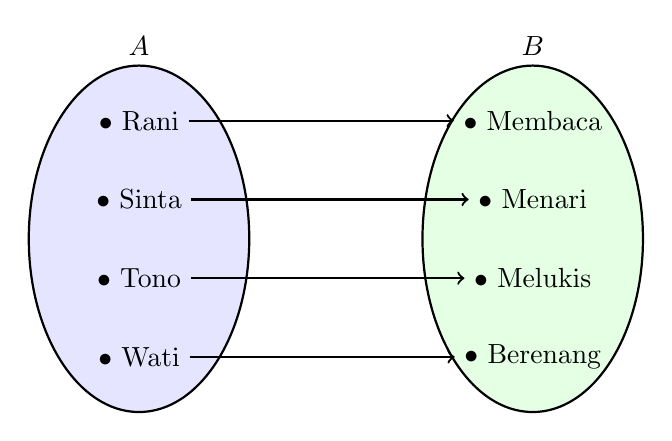
\begin{tikzpicture}[scale=1]
  \draw[thick, fill=blue!10] (0,0) ellipse (1.4 and 2.2);
  \draw[thick, fill=green!10] (5,0) ellipse (1.4 and 2.2);
  \node[above] at (0,2.2) {$A$};
  \node[above] at (5,2.2) {$B$};
  \node (a1) at (0,1.5) {$\bullet$ Rani};
  \node (a2) at (0,0.5) {$\bullet$ Sinta};
  \node (a3) at (0,-0.5) {$\bullet$ Tono};
  \node (a4) at (0,-1.5) {$\bullet$ Wati};
  \node (b1) at (5,1.5) {$\bullet$ Membaca};
  \node (b2) at (5,0.5) {$\bullet$ Menari};
  \node (b3) at (5,-0.5) {$\bullet$ Melukis};
  \node (b4) at (5,-1.5) {$\bullet$ Berenang};
  \draw[->, thick] (a1) -- (b1);
  \draw[->, thick] (a2) -- (b2);
  \draw[->, thick] (a3) -- (b3);
  \draw[->, thick] (a4) -- (b4);
\end{tikzpicture}
\end{center}

\subsection*{Fungsi ``setengah dari''}
$A = \lbrace 1, 2, 3, 4 \rbrace$,
$B = \lbrace 2, 4, 6, 8 \rbrace$:
$1 \to 2$, $2 \to 4$, $3 \to 6$, $4 \to 8$.
Setiap anggota $A$ tepat satu panah keluar, jadi relasi ini fungsi.
\begin{center}
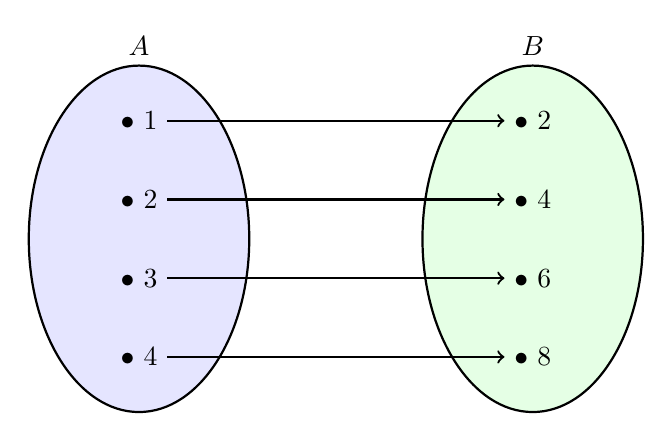
\begin{tikzpicture}[scale=1]
  \draw[thick, fill=blue!10] (0,0) ellipse (1.4 and 2.2);
  \draw[thick, fill=green!10] (5,0) ellipse (1.4 and 2.2);
  \node[above] at (0,2.2) {$A$};
  \node[above] at (5,2.2) {$B$};
  \node (a1) at (0,1.5) {$\bullet$ 1};
  \node (a2) at (0,0.5) {$\bullet$ 2};
  \node (a3) at (0,-0.5) {$\bullet$ 3};
  \node (a4) at (0,-1.5) {$\bullet$ 4};
  \node (b1) at (5,1.5) {$\bullet$ 2};
  \node (b2) at (5,0.5) {$\bullet$ 4};
  \node (b3) at (5,-0.5) {$\bullet$ 6};
  \node (b4) at (5,-1.5) {$\bullet$ 8};
  \draw[->, thick] (a1) -- (b1);
  \draw[->, thick] (a2) -- (b2);
  \draw[->, thick] (a3) -- (b3);
  \draw[->, thick] (a4) -- (b4);
\end{tikzpicture}
\end{center}

\subsection*{Bukan fungsi: satu anggota bercabang}
Relasi hobi yang sama, tetapi Sinta gemar menari dan melukis.
Dari titik Sinta keluar dua panah, jadi relasi ini bukan fungsi.
\begin{center}
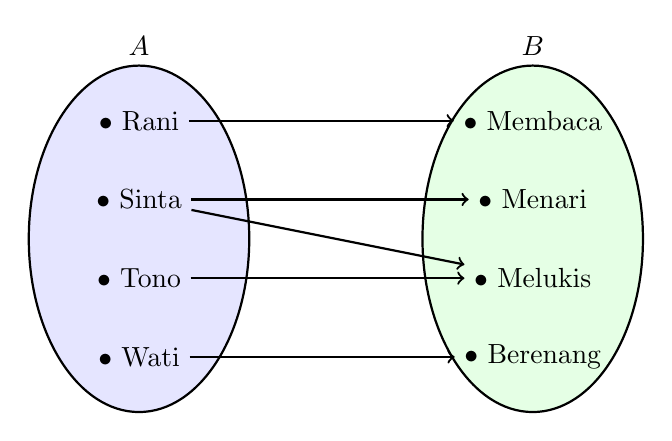
\begin{tikzpicture}[scale=1]
  \draw[thick, fill=blue!10] (0,0) ellipse (1.4 and 2.2);
  \draw[thick, fill=green!10] (5,0) ellipse (1.4 and 2.2);
  \node[above] at (0,2.2) {$A$};
  \node[above] at (5,2.2) {$B$};
  \node (a1) at (0,1.5) {$\bullet$ Rani};
  \node (a2) at (0,0.5) {$\bullet$ Sinta};
  \node (a3) at (0,-0.5) {$\bullet$ Tono};
  \node (a4) at (0,-1.5) {$\bullet$ Wati};
  \node (b1) at (5,1.5) {$\bullet$ Membaca};
  \node (b2) at (5,0.5) {$\bullet$ Menari};
  \node (b3) at (5,-0.5) {$\bullet$ Melukis};
  \node (b4) at (5,-1.5) {$\bullet$ Berenang};
  \draw[->, thick] (a1) -- (b1);
  \draw[->, thick] (a2) -- (b2);
  \draw[->, thick] (a2) -- (b3);
  \draw[->, thick] (a3) -- (b3);
  \draw[->, thick] (a4) -- (b4);
\end{tikzpicture}
\end{center}

\end{document}
